\section{Risultati}
I risultati ottenuti tramite Matlab sono stati valutati in termini di coerenza con 
le nozioni teoriche esposte fino ad ora. In particolare, si discuterà a proposito di:
\begin{itemize}
    \item confronto tra gli output dei due algoritmi descritti;
    \item confronto tra i tempi di esecuzione dei due algoritmi;
    \item quantità ottenute nel calcolo delle osservabili, con i rispettivi errori;
\end{itemize}

\subsection*{Correttezza dell'algoritmo HK}
Come anticipato, la correttezza dell'algoritmo implementato è stata definita rispetto 
all'output dell'algoritmo $A$, che funge quindi da riferimento.
Sono stati eseguiti molti test con vari parametri di input, ma ogni volta 
``fissando'' il reticolo, per avere un confronto sulla stessa struttura.
In Fig. \ref{fig:compare_threshold} viene mostrato un confronto dei valori 
ottenuti tramite i due algoritmi, variando sia la dimensione del reticolo (ogni linea
rappresenta le esecuzioni a dimensione fissata), sia la probabilità di occupazione.
Quest'ultima è considerata un parametro di input per una funzione $f(x)$ ed è
quindi riscontrabile sull'asse delle ascisse. 
\begin{figure}[ht]
    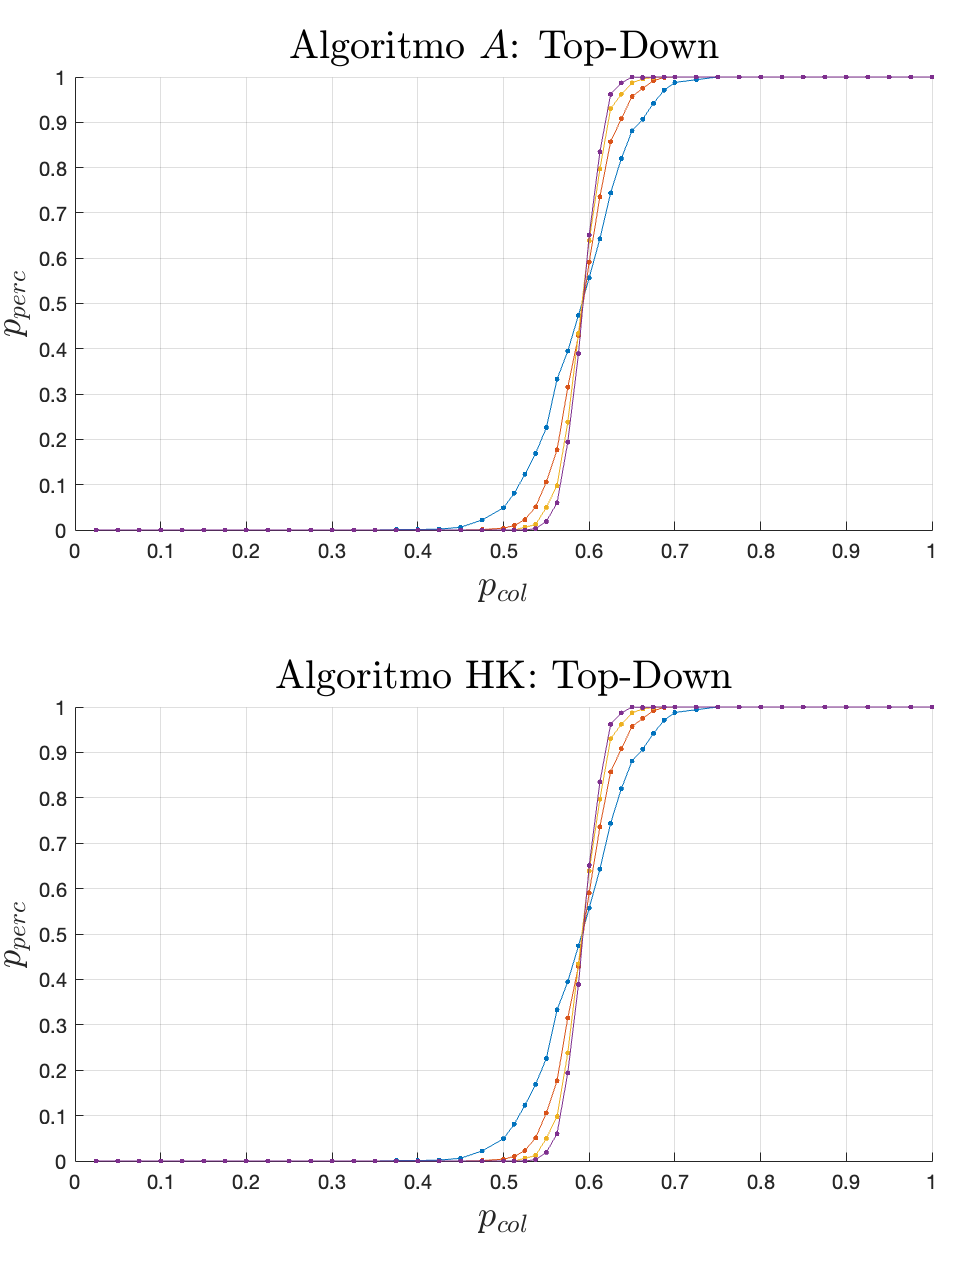
\includegraphics[width=\columnwidth]{compare_threshold_1.png}
    \caption{Confronto tra le frequenze di percolazione top-down ottenute nell'esecuzione
    dei due algoritmi.}
    \label{fig:compare_threshold}
\end{figure}
Risulta interessante eseguire un confronto con la Fig. \ref{fig:threshold} 
relativa al reticolo di taglia infinita: per dimensioni del reticolo più grandi, ci 
si avvicina infatti al suddetto grafico.
Un'altra caratteristica importante da verificare è che le frequenze di 
percolazione top-down registrate coincidano con quelle left-right, nel limite 
dell'errore commesso. Le modalità di svolgimento sono le stesse, con l'aggiunta 
delle misurazioni dell'errore, calcolato come radice quadrata della quantità 
$D_{f_{perc}}$ descritta nell'Eq. \ref{eq:d_f_perc}.
Nel grafico in Fig. \ref{fig:th_errors} viene mostrato un confronto tra i valori 
ottenuti nei due casi con l'algoritmo HK. Ciò che balza all'occhio è la 
superiorità degli errori intorno a $0.6$, valore in cui, tra l'altro, 
si osserva una crescita piuttosto rapida della frequenza di percolazione.
Si compone di 3 iterazioni: una per variare la 
taglia del reticolo, una per variare la probabilità di occupazione e un'ultima per 
eseguire un numero sufficiente di esperimenti perché i risultati siano significativi.
Le frequenze dei due algoritmi sono calcolate con metodi diversi ma equivalenti:
nel primo caso si ``conta'' quante volte la variabile caratteristica ha assunto valore 1
e si divide il totale per il numero di esperimenti $N$; nel secondo caso si utilizza la 
funzione built-in di Matlab \texttt{mean(x)}, che svolge gli stessi passaggi.
Il Cod. \ref{cod:compare} mostra le istruzioni in Matlab per calcolare le quantità 
mostrate nei due grafici. 
\begin{figure}[ht]
    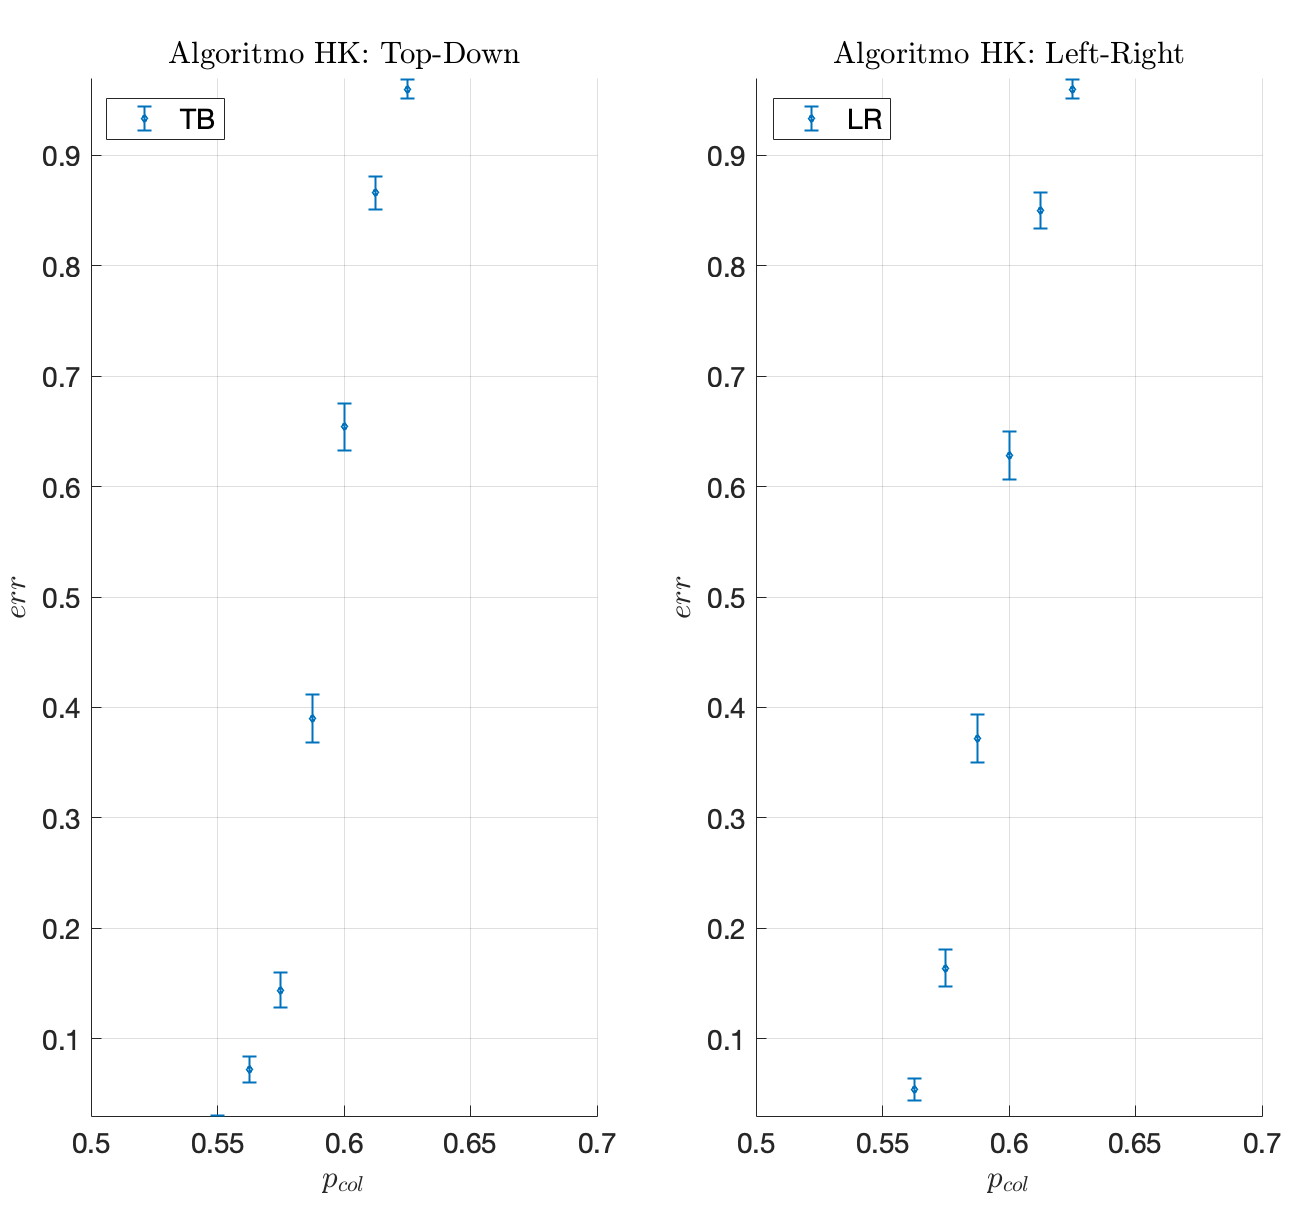
\includegraphics[width=\columnwidth]{errors.png}
    \caption{Confronto tra le frequenze di percolazione top-down e left-right,
    con rispettivi errori.}
    \label{fig:th_errors}
\end{figure}
\begin{lstlisting}[caption={Porzione di codice relativa al confronto tra algoritmi e 
    alla frequenza di percolazione top-down e left-right.}, label={cod:compare}]
for ij = 1:length(L)
    for ii = 1:length(p)
        pp = p(ii);
        s3TB = 0;
        s3LR = 0;
        sHKTB = 0;
        sHKLR = 0;
        espTB = zeros(N,1);
        espLR = zeros(N,1);
        for j = 1:N
            ret = rand(L(ij))<pp;
            res3 = CercaCluster3(ret);
            resHK = CercaClusterHK(ret);

            s3TB = s3TB + res3.percolazioneTB;
            s3LR = s3LR + res3.percolazioneLR;
            espTB(j) = resHK.percolazioneTB;
            espLR(j) = resHK.percolazioneLR;
        end

        probPercTB3(ij,ii) = s3TB / N;
        probPercLR3(ij,ii) = s3LR / N;
        probPercTBHK(ij,ii) = mean(espTB);
        probPercLRHK(ij,ii) = mean(espLR);
        erroreTB(ij,ii) = std(espTB) / sqrt(N);
        erroreLR(ij,ii) = std(espLR) / sqrt(N);
    end
end
\end{lstlisting}

\subsection*{Calcolo delle osservabili}
Lo stesso procedimento necessario per calcolare la frequenza di percolazione è stato svolto per 
le altre osservabili. In Fig. \ref{fig:distributions} si possono riscontrare i comportamenti 
attesi, descritti nella sezione precedente.
Anche in questo caso, viene acclusa l'implementazione in Matlab nel Cod. \ref{cod:distributions}.
Insieme alle quantità, vengono calcolati anche i rispettivi errori, con tecniche analoghe a quanto visto 
fin ora. Per queste quantità valgono le stesse considerazioni fatte sulla natura di $f_{perc}$,
legate alla validità della media e varianza garantita per mezzo di 
TLC e Legge dei Grandi Numeri.
\begin{figure}[ht]
    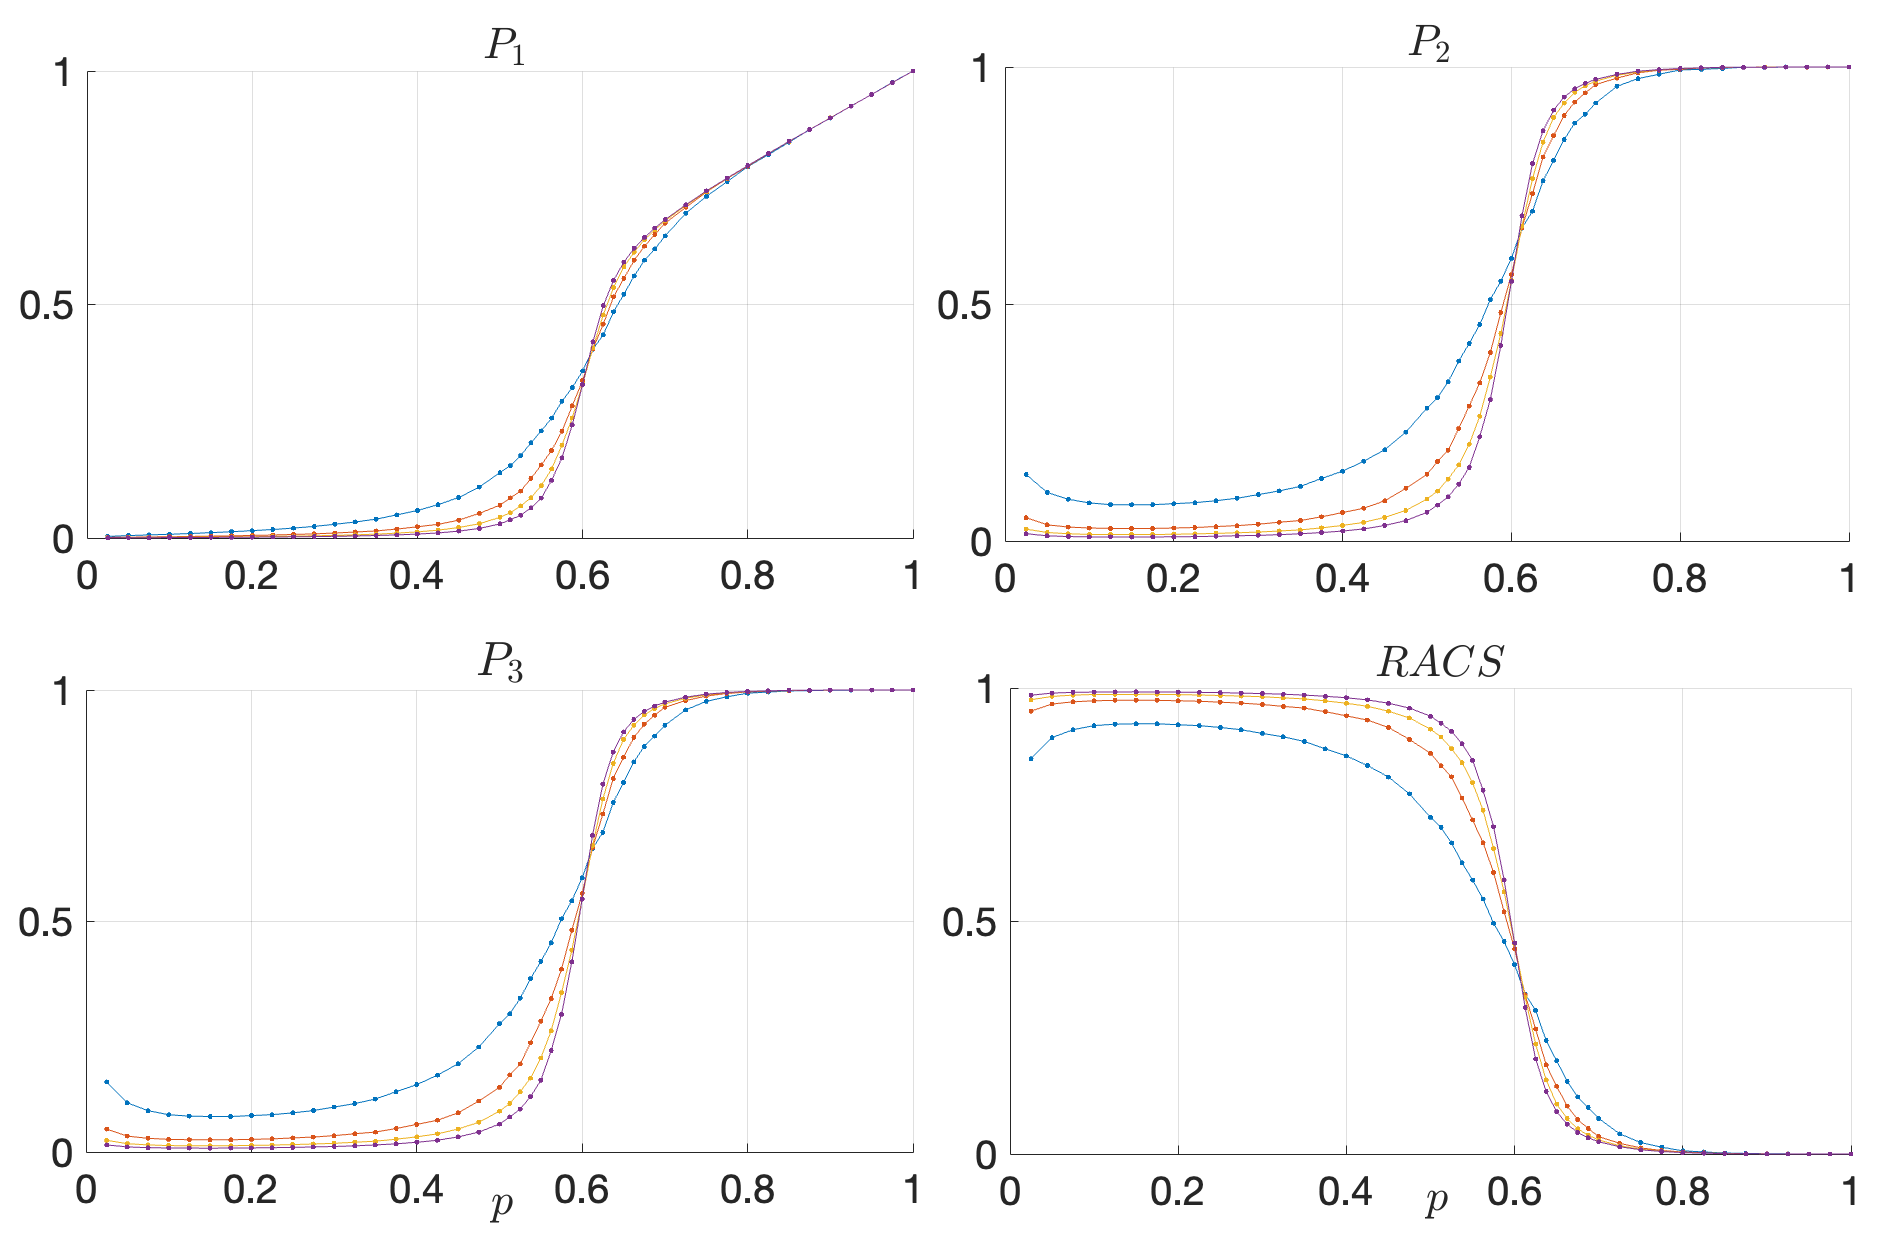
\includegraphics[width=\columnwidth]{p1p2p3racs_3.png}
    \caption{Distribuzioni delle osservabili calcolate in $N=1000$ esperimenti al variare dei parametri.}
    \label{fig:distributions}
\end{figure}
\begin{lstlisting}[caption={Porzione di codice per il calcolo delle osservabili.},label={cod:distributions}]
for ij = 1:length(L)
    for ii = 1:length(p)
        pp = p(ii);
        for j = 1:N
            ret = rand(L(ij))<pp;
            resHK = CercaClusterHK(ret);

            MYsz(ij,j,ii) = mean(resHK.cluSz);
            MYmaxSz(ij,j,ii) = max(resHK.cluSz);
            MYnumCLU(ij,j,ii) = length(resHK.cluSz);
            MYnumCol(ij,j,ii) = sum(resHK.cluSz);
        end
    end
   
    sMax=squeeze(MYmaxSz(ij,:,:));
    P1=sMax./L(ij)^2;
    errore1=std(P1)./sqrt(length(P1));
    P1=mean(P1);

    P2=sMax./(p*L(ij)^2);
    errore2=std(P2)./sqrt(length(P2));
    P2=mean(P2);

    occupied=squeeze(MYnumCol(ij,:,:));
    P3=sMax./occupied;
    P3=squeeze(P3);
    errore3=std(P3)./sqrt(size(P3,2));
    P3=mean(P3);

    occupiedReduced = squeeze(MYnumCol(ij,:,:)-MYmaxSz(ij,:,:));
    racs=occupiedReduced./occupied;
    erroreRacs=std(racs)/sqrt(length(racs));
    racs=mean(racs);
end
\end{lstlisting}

\subsection*{Tempi di esecuzione}